Een Linux server die ge\"installeerd is zonder grafische interface heeft op zijn monitor de prompt Login: daar kan je
inloggen als gebruiker. Via de toets combinatie ALT en F1-F6 kan je schakelen naar verschillende consoles zodat je
meerdere keren ingelogd kan zijn.

Als je werkt vanuit een grafische interface kan je gebruik maken van de Terminal of Terminal Emulator applicatie. Deze brengt je bij de command line interface, zie figuur \ref{fig:DashTerminal}

\begin{figure}
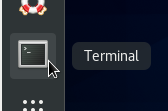
\includegraphics{linuxreader-img021.png}
	\label{fig:DashTerminal}
	\caption{Terminal op de Dash}
\end{figure}

